% Generated from the public primitive catalog. Original Atlas drawing; Apache-2.0.
% Target: sm2-key-exchange-sm3-256; view: overview
\documentclass[border=9pt]{standalone}
% Original Atlas figure theme. Apache-2.0; see the repository LICENSE.
\usepackage[T1]{fontenc}
\usepackage{lmodern}
\usepackage{amsmath,amssymb}
\usepackage{tikz}
\usetikzlibrary{arrows.meta,positioning,calc,fit,backgrounds,decorations.pathreplacing,matrix}
\definecolor{atlasInk}{HTML}{172235}
\definecolor{atlasTeal}{HTML}{0D7B7D}
\definecolor{atlasMuted}{HTML}{637278}
\definecolor{atlasFill}{HTML}{EAF4F2}
\definecolor{atlasLine}{HTML}{B6C8C7}
\tikzset{
  every picture/.style={line width=.65pt,draw=atlasInk,>=Latex},
  every node/.style={text=atlasInk,font=\sffamily\small},
  box/.style={draw,rounded corners=1.5pt,minimum height=.9cm,minimum width=1.6cm,align=center,inner sep=6pt,fill=white},
  accent/.style={box,draw=atlasTeal,fill=atlasFill},
  wire/.style={->,line width=.7pt},
  keywire/.style={wire,draw=atlasTeal,dashed},
  xor/.style={draw,circle,fill=white,inner sep=0pt,minimum size=.38cm},
  add/.style={draw,rectangle,fill=white,inner sep=0pt,minimum size=.38cm},
  note/.style={font=\sffamily\scriptsize,text=atlasMuted,align=center},
  phase/.style={font=\sffamily\small\bfseries,text=atlasTeal},
  group/.style={draw=atlasLine,dashed,rounded corners=2pt,inner sep=8pt}
}
\newcommand{\rotl}{\mathbin{\lll}}
\newcommand{\rotr}{\mathbin{\ggg}}
\newcommand{\kx}{\operatorname{Keccak}\!\text{-}\!f[1600]}

\newcommand{\AtlasModulusBits}{b}
\newcommand{\AtlasFieldBits}{256}
\newcommand{\AtlasHash}{\textsf{SM3}}
\newcommand{\AtlasCurve}{\textsf{curveSM2}}
\newcommand{\AtlasDhGroup}{\textsf{X25519 / X448}}
\newcommand{\AtlasDhPublicA}{\operatorname{XDH}(a,u_0)}
\newcommand{\AtlasDhPublicB}{\operatorname{XDH}(b,u_0)}
\newcommand{\AtlasDhSharedA}{\operatorname{XDH}(a,B)}
\newcommand{\AtlasDhSharedB}{\operatorname{XDH}(b,A)}
\newcommand{\AtlasSaltBytes}{s}
\newcommand{\AtlasSharedBits}{256}
\newcommand{\AtlasPublicKeyBytes}{|pk|}
\newcommand{\AtlasSecretKeyBytes}{|sk|}
\newcommand{\AtlasCiphertextBytes}{|c|}
\newcommand{\AtlasSignatureBytes}{|\sigma|}
\newcommand{\AtlasModuleRank}{k}
\newcommand{\AtlasMatrixRows}{k}
\newcommand{\AtlasMatrixColumns}{\ell}
\newcommand{\AtlasHypertreeHeight}{h}
\newcommand{\AtlasHypertreeLayers}{d}
\newcommand{\AtlasForsHeight}{a}
\newcommand{\AtlasForsTrees}{k}
\newcommand{\AtlasHashBytes}{n}
\newcommand{\AtlasHashFamily}{\textsf{SHA2 / SHAKE}}
\begin{document}
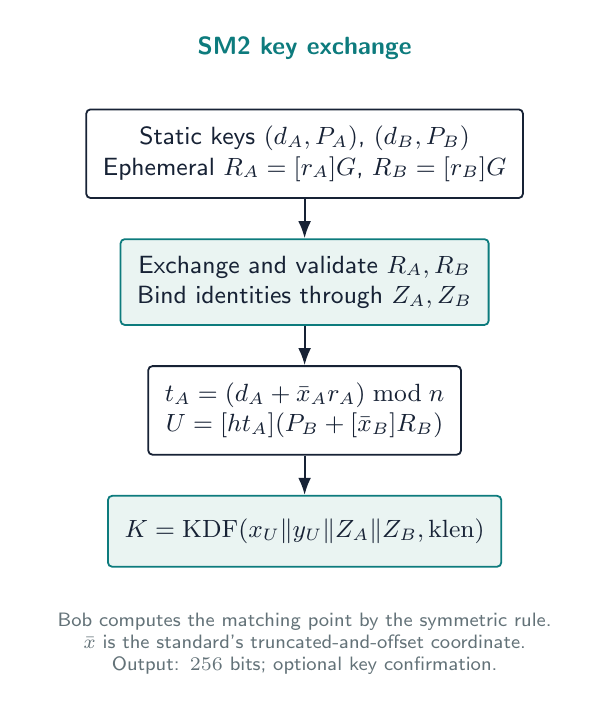
\begin{tikzpicture}[node distance=.5cm]
  \node[phase] (title) {SM2 key exchange};
  \node[box,below=of title] (keys) {Static keys $(d_A,P_A)$, $(d_B,P_B)$\\Ephemeral $R_A=[r_A]G$, $R_B=[r_B]G$};
  \node[accent,below=of keys] (exchange) {Exchange and validate $R_A,R_B$\\Bind identities through $Z_A,Z_B$};
  \node[box,below=of exchange] (combine) {$t_A=(d_A+\bar{x}_A r_A)\bmod n$\\$U=[h t_A](P_B+[\bar{x}_B]R_B)$};
  \node[accent,below=of combine] (derive) {$K=\operatorname{KDF}(x_U\Vert y_U\Vert Z_A\Vert Z_B,\mathrm{klen})$};
  \draw[wire] (keys) -- (exchange); \draw[wire] (exchange) -- (combine); \draw[wire] (combine) -- (derive);
  \node[note,below=.45cm of derive,text width=6.8cm] {Bob computes the matching point by the symmetric rule.\\$\bar{x}$ is the standard's truncated-and-offset coordinate.\\Output: $\AtlasSharedBits$ bits; optional key confirmation.};
\end{tikzpicture}

\end{document}
